% !TEX TS–program = pdflatexmk
% !TeX program used: pdftex

\documentclass[12pt]{beamer}
\usepackage[french]{babel}
\usepackage[utf8]{inputenc}
\usepackage[T1]{fontenc}
\usepackage{url}
\usepackage{graphicx}
\usepackage{subcaption}

\usetheme{Madrid}
%\usetheme{Marburg}
%\usetheme{Frankfurt}
\useoutertheme{split}
\setbeamertemplate{navigation symbols}{}
\usepackage[orientation=landscape,size=custom,width=16,height=9,scale=0.5,debug]{beamerposter} 
%\usepackage{enumitem}
\usepackage{ragged2e}
\usepackage{color}
\let\olditem\item
\renewcommand\item{\olditem\justifying}

\usepackage{natbib}
%\bibliographystyle{ieeetr}
\addbibresource{references.bib}

\setbeamerfont{footnote}{size=\tiny} %reduce the size of the footnote citation

\setbeamertemplate{bibliography item}{\insertbiblabel}  % Add numbered list of references in the end

\begin{document}  
	\author[Melet David CHIRINO CAICEDO]{Melet David CHIRINO CAICEDO \\ Tuteur \\ Yann LABIT}
	\title{\textbf{Linky4Teens}}
	%\subject{}
	%\subtitle{}
	%\logo{}
	\institute{\normalsize{Université Toulouse III Paul Sabatier}}
	%\date{}
	%\subject{KTU Sponsored FDP \\ on \\ Power System Security \& Internet of Things : A Future Energy Scenario}
	%\setbeamercovered{transparent}
	%\setbeamertemplate{navigation symbols}{}
	\begin{frame}[plain]
		\vspace*{5pt}
		\centering{\textbf{Stage 3 mois \\ du \\ M1 Systèmes Embarqués}}\\
		%\centering{\texttt{College of Engineering Trivandrum}}
		\vspace*{10pt}
		\maketitle
	\end{frame}

\begin{frame}
\frametitle{Definition du projet}
Le projet Linky4Teens cherche à améliorer la performance des jeunes athlètes. J'ai travaillé pour developper des protypes des appareils 
	\begin{figure}
		\centering
		\includegraphics[width=0.36\textwidth]{"images/starting_bloc"}
		\label{fig:starting_bloc}
	\end{figure}
	\begin{figure}
		\centering
		\includegraphics[width=0.36\textwidth]{"images/starting_bloc"}
		\label{fig:starting_bloc}
	\end{figure}

\begin{itemize}
	\item A network of items — each embedded with sensors — which are connected to the Internet. \footfullcite{minerva2015towards}

	\item The interconnection via the internet of computing devices embedded in everyday objects, enabling them to send and receive data. \footfullcite{lexico}
\end{itemize}

\begin{figure}
	\centering
	\subfigure[Schéma du circuit]{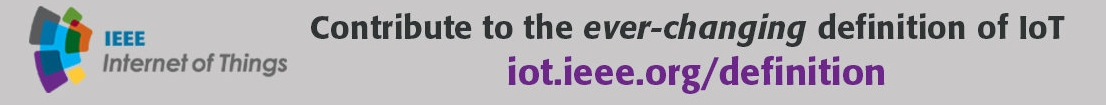
\includegraphics [height=2in]{images/IoTDefinitionsBanner_v2}
	\label{img:eagle:schema}}
	% 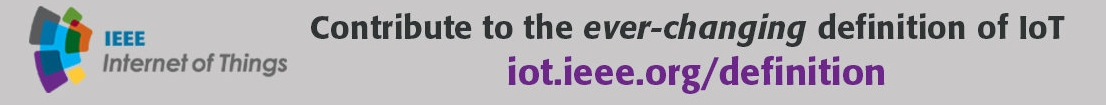
\includegraphics[width=0.9\linewidth]{images/IoTDefinitionsBanner_v2}
	\label{fig:iotdefinitionsbannerv2}
\end{figure}
\end{frame}

\begin{frame}{Internet of Things - Milestones}
	\begin{itemize}
		\item 1969 - ARPANET
		\item 1980's - Commercial Internet services
		\item 1993 - Global Positioning System
		\item 2017 - IPv6 Standard
	\end{itemize}
\vspace*{10pt}
IPv6 - 128 bit addresses as opposed to 32 bit addresses in IPv4 \\
$2^{128} =  3.4 * 10^{38}$  addresses \\
	
\end{frame}

\begin{frame}{The first's in IoT }
	\begin{columns}
		\begin{column}{0.5\textwidth}
			\begin{itemize}
				\item 1982 - World’s first IoT device - Carnegie Mellon University, School of Computer Science,USA
				\item Toaster (1990), Webcam/Coffee pot(1993).........
				\item LG Internet Digital DIOS (2000) - First Internet Refrigerator 
		\end{itemize}
		\end{column}
			
		\begin{column}{0.5\textwidth}
		\begin{figure}
			\centering
			\includegraphics[width=0.8\linewidth]{"images/cmu internet-coke-machine"}
			\\ CMU SCS connected coke machine		\label{fig:cmu-internet-coke-machine}
		\end{figure}
		\end{column}
	\end{columns}
\footfullcite{cmu}, \footfullcite{cmu2}, \footfullcite{lg}
\end{frame}

\begin{frame}{Comparison of RF technologies}
	\begin{figure}
		\centering
		\includegraphics[width=0.98\textwidth]{"images/iot rf"}
		\label{fig:iot rf}
	\end{figure}
	\footfullcite{ray2018survey}	
\end{frame}

\end{document}
